% Charla de avances (unos 10 minutos) con los docentes que forman parte del proyecto y aportaron los corpus.
% Centrada en la ontología (OHAC), el tesauro y cómo se construye y usa el grafo. El guion de lo que se dice en
% cada diapositiva está en guion_charla.md; el respaldo con todo el detalle, en proyecto.tex.
% Compilar:  python scripts/cifras.py && python scripts/datos_presentacion.py && latexmk -pdf avances.tex
% Ninguna cifra de los datos se escribe a mano (../articulo/cifras.tex y datos_proyecto.tex).
\documentclass[aspectratio=169,10pt]{beamer}
\usetheme{metropolis}
\metroset{block=fill,numbering=fraction,progressbar=frametitle}
\usepackage[T1]{fontenc}
\usepackage[utf8]{inputenc}
\usepackage[spanish,es-noshorthands,es-tabla,es-nodecimaldot]{babel}
\usepackage{booktabs}
\usepackage{array}
\newcolumntype{L}[1]{>{\raggedright\arraybackslash}p{#1}}
\usepackage{graphicx}
\usepackage{tikz}
\usetikzlibrary{positioning,arrows.meta,calc,fit,babel}
\usepackage{csquotes}
% GENERADO por scripts/cifras.py. No editar a mano: ejecutar el script.
% Lo cargan articulo/main.tex y presentacion/main.tex.
\newcommand{\cifraAfirmaciones}{504}
\newcommand{\cifraAlineaciones}{66}
\newcommand{\cifraAtributos}{30}
\newcommand{\cifraCandidatos}{19}
\newcommand{\cifraCatalogoRegistros}{66}
\newcommand{\cifraCitas}{1\,049}
\newcommand{\cifraClases}{41}
\newcommand{\cifraConceptos}{164}
\newcommand{\cifraDUnoEspurias}{285}
\newcommand{\cifraDSeisAfirmaciones}{504}
\newcommand{\cifraDSeisNegaciones}{20}
\newcommand{\cifraDefinicionesDeTrabajo}{22}
\newcommand{\cifraEntidadesNoPersona}{260}
\newcommand{\cifraEntidadesSinTipo}{135}
\newcommand{\cifraEsquemas}{12}
\newcommand{\cifraExpedientes}{1}
\newcommand{\cifraFormas}{50}
\newcommand{\cifraGrafos}{77}
\newcommand{\cifraHechosEnlazados}{13}
\newcommand{\cifraHechosNarrados}{61}
\newcommand{\cifraMenciones}{545}
\newcommand{\cifraMencionesEnlazadas}{123}
\newcommand{\cifraMutacionesDeclaradas}{36}
\newcommand{\cifraNegaciones}{20}
\newcommand{\cifraNegacionesConRespuesta}{4}
\newcommand{\cifraPiezas}{33}
\newcommand{\cifraPreguntas}{20}
\newcommand{\cifraPropiedades}{75}
\newcommand{\cifraRazonadorCierre}{189\,555}
\newcommand{\cifraRazonadorInconsistencias}{0}
\newcommand{\cifraRazonadorTripletas}{56\,351}
\newcommand{\cifraReconstrucciones}{35}
\newcommand{\cifraReconstruccionesConFechas}{36}
\newcommand{\cifraTerminosPropios}{0}
\newcommand{\cifraTripletas}{31\,037}
\newcommand{\cifraValoresLiterales}{211}

% Generado por scripts/datos_presentacion.py. No editar a mano.
\newcommand{\serieClases}{(0,53) (1,18) (2,16) (3,15) (4,13) (5,3)}
\newcommand{\rotulosClases}{{persona},{lugar},{cosa},{grupo},{hecho},{cargo}}
\newcommand{\serieCreencia}{(0,29) (1,70) (2,16) (3,2) (4,1)}
\newcommand{\rotulosCreencia}{{verdadero},{probable},{posible},{improbable},{indeterminado}}
\newcommand{\serieFuerza}{(0,249) (1,86) (2,53) (3,52) (4,43) (5,21)}
\newcommand{\rotulosFuerza}{{testimonial},{informativa},{resolutiva},{alegación de parte},{dictaminadora},{fedataria}}
\newcommand{\serieFuerzaX}{(249,0) (86,1) (53,2) (52,3) (43,4) (21,5)}
\newcommand{\datoAfirma}{484}
\newcommand{\datoNiega}{20}
\newcommand{\seriePiezas}{(0,36) (1,5) (2,30) (3,29) (4,19) (5,52) (6,26) (7,4) (8,16) (9,11) (10,5) (11,1) (12,7) (13,17) (14,7) (15,3) (16,22) (17,24) (18,19) (19,49) (20,6) (21,31) (22,6) (23,3) (24,42) (25,9) (26,17) (27,4) (28,4)}
\newcommand{\rotulosPiezas}{{P01},{P02},{P03},{P04},{P05},{P06},{P07},{P08},{P09},{P10},{P11},{P12},{P13},{P14},{P16},{P17},{P18},{P19},{P20},{P21},{P22},{P23},{P24},{P25},{P27},{P28},{P29},{P30},{P31}}
\newcommand{\nPiezasConAfirmaciones}{29}
\newcommand{\serieAgenteCompleta}{(0,3) (1,5) (2,5) (3,7) (4,8) (5,3) (6,0)}
\newcommand{\serieAgenteEsencial}{(0,3) (1,11) (2,12) (3,10) (4,12) (5,9) (6,0)}
\newcommand{\serieAgenteForma}{(0,14) (1,17) (2,19) (3,17) (4,18) (5,12) (6,0)}
\newcommand{\serieAgenteVerificada}{(0,19) (1,19) (2,18) (3,18) (4,19) (5,15) (6,0)}
\newcommand{\rotulosAgente}{{v1},{h1},{h2},{r1},{r2},{r3},{r4}}
\newcommand{\tablaAgente}{%
v1 & 20 & 3 & 3 & 14 & 19 & 25\,k \\
h1 & 20 & 5 & 11 & 17 & 19 & 36\,k \\
h2 & 20 & 5 & 12 & 19 & 18 & 31\,k \\
r1 & 20 & 7 & 10 & 17 & 18 & 31\,k \\
r2 & 20 & 8 & 12 & 18 & 19 & 33\,k \\
r3 & 15 & 3 & 9 & 12 & 15 & 27\,k \\
r4 & 0 & 0 & 0 & 0 & 0 & 0\,k \\
}
\newcommand{\mediaCompleta}{7,5}
\newcommand{\numCompleta}{7.50}
\newcommand{\desvCompleta}{0,5}
\newcommand{\mediaEsencial}{11,0}
\newcommand{\numEsencial}{11.00}
\newcommand{\desvEsencial}{1,0}
\newcommand{\mediaForma}{17,5}
\newcommand{\numForma}{17.50}
\newcommand{\desvForma}{0,5}
\newcommand{\mediaVerificada}{18,5}
\newcommand{\numVerificada}{18.50}
\newcommand{\desvVerificada}{0,5}
\newcommand{\nEjecucionesLlenas}{2}
\newcommand{\matrizEsencial}{(0,0) [1] (1,0) [0] (2,0) [0] (3,0) [0] (4,0) [0] (5,0) [0] (6,0) [0] (7,0) [0] (8,0) [0] (9,0) [0] (10,0) [0] (11,0) [0] (12,0) [0] (13,0) [0] (14,0) [1] (15,0) [0] (16,0) [0] (17,0) [0] (18,0) [0] (19,0) [1] (0,1) [1] (1,1) [0] (2,1) [1] (3,1) [1] (4,1) [1] (5,1) [0] (6,1) [0] (7,1) [1] (8,1) [1] (9,1) [0] (10,1) [0] (11,1) [1] (12,1) [0] (13,1) [1] (14,1) [1] (15,1) [0] (16,1) [1] (17,1) [0] (18,1) [1] (19,1) [0] (0,2) [1] (1,2) [0] (2,2) [1] (3,2) [1] (4,2) [1] (5,2) [0] (6,2) [0] (7,2) [0] (8,2) [1] (9,2) [1] (10,2) [1] (11,2) [0] (12,2) [0] (13,2) [1] (14,2) [1] (15,2) [0] (16,2) [1] (17,2) [0] (18,2) [1] (19,2) [1] (0,3) [1] (1,3) [0] (2,3) [1] (3,3) [1] (4,3) [1] (5,3) [0] (6,3) [0] (7,3) [0] (8,3) [1] (9,3) [0] (10,3) [0] (11,3) [0] (12,3) [0] (13,3) [1] (14,3) [1] (15,3) [0] (16,3) [0] (17,3) [1] (18,3) [1] (19,3) [1] (0,4) [1] (1,4) [0] (2,4) [1] (3,4) [1] (4,4) [1] (5,4) [0] (6,4) [0] (7,4) [0] (8,4) [1] (9,4) [0] (10,4) [1] (11,4) [1] (12,4) [0] (13,4) [1] (14,4) [1] (15,4) [0] (16,4) [0] (17,4) [1] (18,4) [1] (19,4) [1] (0,5) [1] (1,5) [0] (2,5) [1] (3,5) [1] (4,5) [1] (5,5) [0] (6,5) [0] (7,5) [0] (8,5) [1] (9,5) [0] (10,5) [1] (11,5) [1] (12,5) [0] (13,5) [1] (14,5) [1] (15,5) [-1] (16,5) [-1] (17,5) [-1] (18,5) [-1] (19,5) [-1] (0,6) [-1] (1,6) [-1] (2,6) [-1] (3,6) [-1] (4,6) [-1] (5,6) [-1] (6,6) [-1] (7,6) [-1] (8,6) [-1] (9,6) [-1] (10,6) [-1] (11,6) [-1] (12,6) [-1] (13,6) [-1] (14,6) [-1] (15,6) [-1] (16,6) [-1] (17,6) [-1] (18,6) [-1] (19,6) [-1]}
\newcommand{\maxEjecucion}{6}
\newcommand{\pcSiempreBien}{01, 03, 04, 05, 09, 14, 15, 19}
\newcommand{\pcSiempreMal}{02, 06, 07, 13, 16}
\newcommand{\pcVariables}{08, 10, 11, 12, 17, 18, 20}
\newcommand{\interCompleta}{10}
\newcommand{\interEsencial}{17}
\newcommand{\interForma}{20}
\newcommand{\interVerificada}{20}


\definecolor{tinta}{HTML}{23373B}
\definecolor{ocre}{HTML}{B5651D}
\definecolor{verde}{HTML}{3F7F4F}
\definecolor{rojo}{HTML}{B3261E}
\definecolor{gris}{HTML}{C9D1D2}
\setbeamercolor{alerted text}{fg=ocre}
\setbeamercolor{progress bar}{fg=ocre}
\newcommand{\cita}[1]{«\textit{#1}»}
\newcommand{\ttt}[1]{\texttt{\small #1}}
\newcommand{\cifra}[1]{\textbf{\alert{#1}}}
\tikzset{
  caja/.style={draw=tinta!60, fill=#1, rounded corners=3pt, align=center, font=\scriptsize, inner sep=3pt},
  caja/.default=white,
  flecha/.style={-{Stealth[length=1.8mm]}, thick, tinta!70},
  rot/.style={font=\tiny, fill=white, inner sep=1pt},
}

\title{Un grafo de conocimiento para expedientes judiciales coloniales}
\subtitle{La ontología OHAC, su tesauro y cómo estamos construyendo el grafo del expediente CC Leg.~14 Exp.~18}
\author{Jhon Jesus Quispe Machaca \and Ian Logan Will Quispe Ventura}
\institute{Laboratorio LAAD · Universidad Nacional de San Antonio Abad del Cusco}
\date{Avances · 25 de noviembre de 2026}

\begin{document}
\maketitle

% ---------------------------------------------------------------------
\begin{frame}{Qué estamos construyendo}
\centering
\begin{tikzpicture}[node distance=9mm]
\node[caja=ocre!15, text width=3.6cm, minimum height=2.3cm] (o) {\footnotesize\textbf{1 · La ontología (OHAC)}\\[3pt]
  cómo se representa un expediente: cuatro capas, un tesauro y reglas de validación};
\node[caja=tinta!10, text width=3.6cm, minimum height=2.3cm, right=of o] (g) {\footnotesize\textbf{2 · El grafo}\\[3pt]
  el expediente piloto (Tinta, 1806) representado con esa ontología: \cifraAfirmaciones{} afirmaciones};
\node[caja=verde!12, text width=3.6cm, minimum height=2.3cm, right=of g] (u) {\footnotesize\textbf{3 · Su uso}\\[3pt]
  consultas, un visor y un agente que responde preguntas citando el expediente};
\draw[flecha] (o) -- (g); \draw[flecha] (g) -- (u);
\end{tikzpicture}

\bigskip
\begin{block}{La idea que guía todo}
Un expediente no registra hechos: registra \alert{quién afirmó qué}, ante quién, en qué actuación y con qué fuerza
procesal. El grafo conserva cada voz y \alert{calcula} dónde chocan; no decide quién tiene razón.
\end{block}
\end{frame}

% ---------------------------------------------------------------------
\begin{frame}{La ontología en una imagen: cuatro capas}
\footnotesize
\begin{tabular}{@{}L{2.7cm}L{3.0cm}L{3.2cm}L{4.4cm}@{}}
\toprule
Capa & Responde a & Estándar & Ejemplo del expediente \\
\midrule
\textbf{1 · Documento} & ¿qué papel es? & RiC-O (ICA) + CIDOC CRM & pieza P18: declaración jurada de Isidro Cano \\
\textbf{2 · Mención} & ¿qué está escrito, y dónde? & PiCo / ROAR + Web Annotation & el nombre «Andres Chuquitapa» en el tramo UT01, tal cual \\
\textbf{3 · Afirmación} & ¿quién dijo qué de quién? & CIDOC CRM (E13) & Cano \alert{niega} que Chuquitapa fuera coronel \\
\textbf{4 · Reconstruc\-ción} & ¿qué propone el investigador? & CRMinf + PiCo & esas grafías son una persona: \emph{probable} \\
\midrule
Procedencia & ¿de dónde sale este dato? & PROV-O & qué transcripción, qué proceso, quién validó \\
\bottomrule
\end{tabular}

\bigskip
\small
\begin{itemize}
\item Cada capa vive en su propio grafo nombrado: no se mezclan.
\item En las capas 1--3 \alert{no hay verdadero ni falso}; una resolución del juez también es una afirmación.
\item Solo la capa 4 lleva creencias, y siempre con autor, fecha y argumento.
\end{itemize}
\end{frame}

% ---------------------------------------------------------------------
\begin{frame}{Un ejemplo que atraviesa las capas}
\centering
\begin{tikzpicture}[x=1cm, y=1cm]
\foreach \y/\t/\c in {3.6/{4 · Recons-\\trucción}/ocre!8, 2.15/{3 · Afir-\\mación}/tinta!8, 0.7/{2 · Mención}/tinta!5, -0.75/{1 · Docu-\\mento}/tinta!3} {
  \fill[\c] (-0.3,\y-0.68) rectangle (13.9,\y+0.68);
  \node[anchor=west, align=left, font=\scriptsize\bfseries, tinta!70, text width=1.5cm] at (-0.25,\y) {\t};
}
\node[caja=white, text width=3.3cm] (p18) at (7.7,-0.75) {Pieza P18 · declaración jurada\\(fuerza: \textbf{testimonial})};
\node[caja=white, text width=2.6cm] (p01) at (12.3,-0.75) {Pieza P01 · certificación\\de agosto};
\node[caja=white] (mc) at (3.3,0.7) {mención «Isidro Cano»\\tramo UT11};
\node[caja=white] (mch) at (7.7,0.7) {mención «Andres Chuquitapa»\\tramo UT01};
\node[caja=tinta!15, text width=4.4cm] (a) at (7.7,2.15) {\textbf{A-UT11-004}: \emph{ejerce-cargo = coronel
  rebelde}\\polaridad \textcolor{rojo}{\textbf{niega}} · cita \cita{Comisionado por este y no coronel}};
\node[caja=tinta!15, text width=2.6cm] (a1) at (12.3,2.15) {\textbf{A-UT01-001}: el mismo Cano \textbf{afirma}
  \cita{complice y coronel}};
\node[caja=ocre!20, text width=4.2cm] (r) at (7.7,3.6) {\textbf{Andrés Chuquitapa}: una persona reconstruida
  con 45 grafías · \emph{probable}};
\node[caja=ocre!20, text width=2.6cm] (rc) at (3.3,3.6) {\textbf{Isidro Cano}\\5 menciones · \emph{verdadero}};
\draw[flecha] (a) -- node[rot, pos=0.5] {quién afirma (declarante)} (mc);
\draw[flecha] (a) -- node[rot] {sobre quién} (mch);
\draw[flecha] (a.east) to[out=-15, in=70] node[rot, pos=0.6] {en qué actuación} (p18.north east);
\draw[flecha, rojo!80] (a) -- node[rot] {responde a} (a1);
\draw[flecha] (a1) -- (p01);
\draw[flecha, dashed, ocre] (r.west) to[out=200, in=160] node[rot, pos=0.3] {reúne} (mch.west);
\draw[flecha, dashed, ocre] (rc.west) to[out=200, in=160] node[rot, pos=0.3] {reúne} (mc.west);
\end{tikzpicture}

\medskip
\footnotesize El grafo no dice si Chuquitapa fue coronel: dice que Cano lo afirmó en agosto y lo negó bajo juramento en
septiembre. La \alert{disputa} se calcula de esas dos afirmaciones.
\end{frame}

% ---------------------------------------------------------------------
\begin{frame}{La afirmación por dentro (capa 3)}
\begin{columns}[T]
\column{0.53\textwidth}
\footnotesize
\textbf{Cada afirmación (\ttt{crm:E13}) guarda:}

\smallskip
\begin{tabular}{@{}L{2.2cm}L{3.9cm}@{}}
\toprule
quién la hace & mención + su rol (declarante, certificante…) \\
en qué actuación & pieza, fecha \emph{escrita}, ante quién, quién firma \\
sobre qué & mención, pieza o hecho narrado \\
qué afirma & un atributo de una lista cerrada (\cifraAtributos) \\
valor & concepto, otra mención o texto \\
polaridad & afirma / niega \\
fundamento & de vista, de oídas, notoriedad… \\
responde a & otra afirmación o \enquote{según otro} \\
cita & copia exacta del tramo \\
\bottomrule
\end{tabular}
\column{0.45\textwidth}
\footnotesize
\textbf{La fuerza la da el tipo de actuación:}

\smallskip
\begin{tabular}{@{}L{2.6cm}L{1.9cm}@{}}
\toprule
certificación, declaración & testimonial \\
petición & de parte \\
informe, oficio & informativa \\
vista fiscal & dictaminadora \\
auto, decreto & resolutiva \\
notificación & fedataria \\
\bottomrule
\end{tabular}

\medskip
Una resolución \alert{obliga en el proceso}, pero no hace verdadero lo resuelto, ni implica que se cumpliera. Por eso
\enquote{¿qué castigo se ejecutó?} se responde \alert{no consta}.
\end{columns}
\end{frame}

% ---------------------------------------------------------------------
\begin{frame}{Identidades: hipótesis con autor y creencia (capa 4)}
\begin{columns}[T]
\column{0.52\textwidth}
\small
\begin{itemize}
\item Nunca se fusionan grafías: \enquote{Guancachoque} y \enquote{Huancachoque} son dos menciones.
\item Decir que son la misma persona es una \alert{reconstrucción} (CRMinf), con:
  \begin{itemize}\footnotesize
  \item autor y fecha;
  \item premisas: las afirmaciones en que se apoya;
  \item argumento escrito;
  \item creencia: verdadero, probable, posible, improbable.
  \end{itemize}
\item Lecturas incompatibles conviven como \alert{rivales}; nadie elige en silencio.
\item Hoy hay \cifraReconstrucciones{} reconstrucciones (personas, lugares, grupos, hechos, cargos), propuestas por un
      modelo de lenguaje y \alert{sin validar}.
\end{itemize}
\column{0.46\textwidth}
\centering
\begin{tikzpicture}[node distance=6mm and 4mm]
\node[caja=tinta!5] (m1) {«Martin Cazorla»\\firma en agosto (P05)};
\node[caja=tinta!5, right=of m1] (m2) {«Mariano Casorla»\\declara en sept. (P19)};
\node[caja=ocre!15, below=13mm of m1] (ra) {A: la misma persona\\\textit{probable}};
\node[caja=ocre!15, below=13mm of m2] (rb) {B: otra persona\\\textit{improbable}};
\draw[flecha] (m1) -- (ra); \draw[flecha] (m2) -- (ra); \draw[flecha] (m2) -- (rb);
\draw[ocre, dashed, thick] (ra) -- node[below, font=\tiny] {rivales} (rb);
\end{tikzpicture}

\medskip
\scriptsize Argumento de A: al declarante se le muestra \cita{la certificación De folio 4 su firma Martin casorla} y
habla de ella en primera persona.
\end{columns}
\end{frame}

% ---------------------------------------------------------------------
\begin{frame}{El tesauro: lo andino y lo procesal como datos}
\begin{columns}[T]
\column{0.5\textwidth}
\footnotesize
\textbf{\cifraEsquemas{} esquemas SKOS, \cifraConceptos{} conceptos}

\smallskip
\begin{tabular}{@{}L{2.6cm}L{3.5cm}@{}}
\toprule
tipos de actuación & certificación, auto, vista fiscal… \\
roles & declarante, receptor, firmante… \\
cargos & cacique, recaudador, segunda… \\
condiciones & originario, forastero, tributario… \\
entidades & ayllu, parcialidad, pueblo… \\
atributos & \cifraAtributos{} cosas que se pueden afirmar \\
polaridad · fuerza · fundamento & afirma/niega; testimonial…; de vista, de oídas… \\
creencias · documentos · anotación & solo capa 4; folio, legajo…; marcas del anotador \\
\bottomrule
\end{tabular}
\column{0.48\textwidth}
\small
\textbf{Decisiones que conviene discutir}
\begin{itemize}\footnotesize
\item \cita{India Ordinaria} se guarda como \emph{ordinario}, \alert{no} como originaria.
\item El \emph{ayllu} es un grupo, no un lugar.
\item \enquote{Gobernador} (UT12.a): cargo con nota de referente dudoso.
\item Un cargo o una condición nunca es un tipo de persona: es algo que \emph{alguien afirma}.
\end{itemize}
\textbf{Cómo crece}
\begin{itemize}\footnotesize
\item Lo nuevo entra como \alert{candidato} (hoy \cifraCandidatos) y un curador lo aprueba o rechaza; nada se borra.
\item \cifraDefinicionesDeTrabajo{} definiciones son \enquote{de trabajo}, sin fuente.
\item Enlaces a Wikidata y Getty solo como \enquote{cercano}, nunca \enquote{igual}.
\end{itemize}
\end{columns}
\end{frame}

% ---------------------------------------------------------------------
\begin{frame}{Estándares, reglas y \cifraTerminosPropios{} términos propios}
\begin{columns}[T]
\column{0.5\textwidth}
\small
\textbf{OHAC es un perfil, no una ontología nueva}
\begin{itemize}\footnotesize
\item Usa términos de RiC-O, CIDOC CRM, CRMinf, PiCo, ROAR, PROV-O, Web Annotation y SKOS.
\item \alert{No inventa clases ni propiedades}: lo local va al tesauro. Se comprueba contra las especificaciones.
\item Por qué: cualquiera que conozca esos estándares lee el grafo sin nuestra documentación, y el modelo no queda
      huérfano cuando el proyecto termine.
\end{itemize}
\textbf{\cifraFormas{} reglas SHACL lo hacen cumplir}, por ejemplo:
\begin{itemize}\footnotesize
\item toda afirmación tiene afirmante, actuación, polaridad, fuerza y cita;
\item ninguna afirmación lleva valor de verdad;
\item ninguna mención se fusiona con otra.
\end{itemize}
\column{0.47\textwidth}
\small
\textbf{Lo que hallamos en los estándares}

\smallskip
\footnotesize Al usarlos con datos reales encontramos 7 defectos. Dos que importan para la historia:
\begin{itemize}\footnotesize
\item CRMinf trata toda afirmación como \enquote{honesta}: cada testimonio hereda una \alert{presunción de sinceridad}
      (\cifraDSeisAfirmaciones{} afirmaciones, \cifraDSeisNegaciones{} de ellas negaciones). Lo documentamos y lo
      contamos.
\item CIDOC CRM vuelve \enquote{actor} a quien afirma, incluso al certificante del que el juez dice \cita{no hay tal
      hombre}. Lo leemos como \enquote{actor tal como consta}.
\end{itemize}
\end{columns}
\end{frame}

% ---------------------------------------------------------------------
\begin{frame}{Cómo se está construyendo el grafo}
\centering
\begin{tikzpicture}[node distance=4mm]
\node[caja=tinta!5, text width=1.9cm] (t) {Transcripción\\paleográfica};
\node[caja=ocre!15, text width=2.3cm, right=of t] (a) {Modelo de lenguaje\\llena \alert{fichas}\\con cita obligatoria};
\node[caja=tinta!5, text width=2cm, right=of a] (v) {Validación:\\cita exacta,\\lista cerrada};
\node[caja=tinta!5, text width=1.9cm, right=of v] (m) {Conversión\\a RDF por código};
\node[caja=tinta!12, text width=1.9cm, right=of m] (g) {Grafo +\\reglas SHACL\\+ razonador};
\draw[flecha] (t) -- (a); \draw[flecha] (a) -- (v); \draw[flecha] (v) -- (m); \draw[flecha] (m) -- (g);
\node[caja=white, text width=2.6cm, below=5mm of v] (h) {Una persona cura las piezas y su tipo de actuación};
\draw[flecha] (h) -| (m);
\end{tikzpicture}

\medskip
\begin{columns}[T]
\column{0.32\textwidth}
\footnotesize
\textbf{El modelo propone}\\ menciones, afirmaciones con su cita, hipótesis de identidad.

\smallskip
\textbf{Nunca decide}\\ tipo de acto, folio, identidad, verdad ni fuerza.
\column{0.3\textwidth}
\footnotesize
\textbf{Hoy, el piloto}\\
\cifraPiezas{} piezas · \cifraMenciones{} menciones\\
\cifraAfirmaciones{} afirmaciones · \cifraReconstrucciones{} reconstrucciones\\
\cifraTripletas{} tripletas
\column{0.34\textwidth}
\footnotesize
\textbf{Validación (sin modelo)}\\
citas exactas: \cifraCitas/\cifraCitas\\
violaciones SHACL: 0 · contradicciones: \cifraRazonadorInconsistencias\\
preguntas de competencia: \cifraPreguntas/\cifraPreguntas
\end{columns}
\end{frame}

% ---------------------------------------------------------------------
\begin{frame}{Qué hacemos con el grafo}
\begin{columns}[T]
\column{0.55\textwidth}
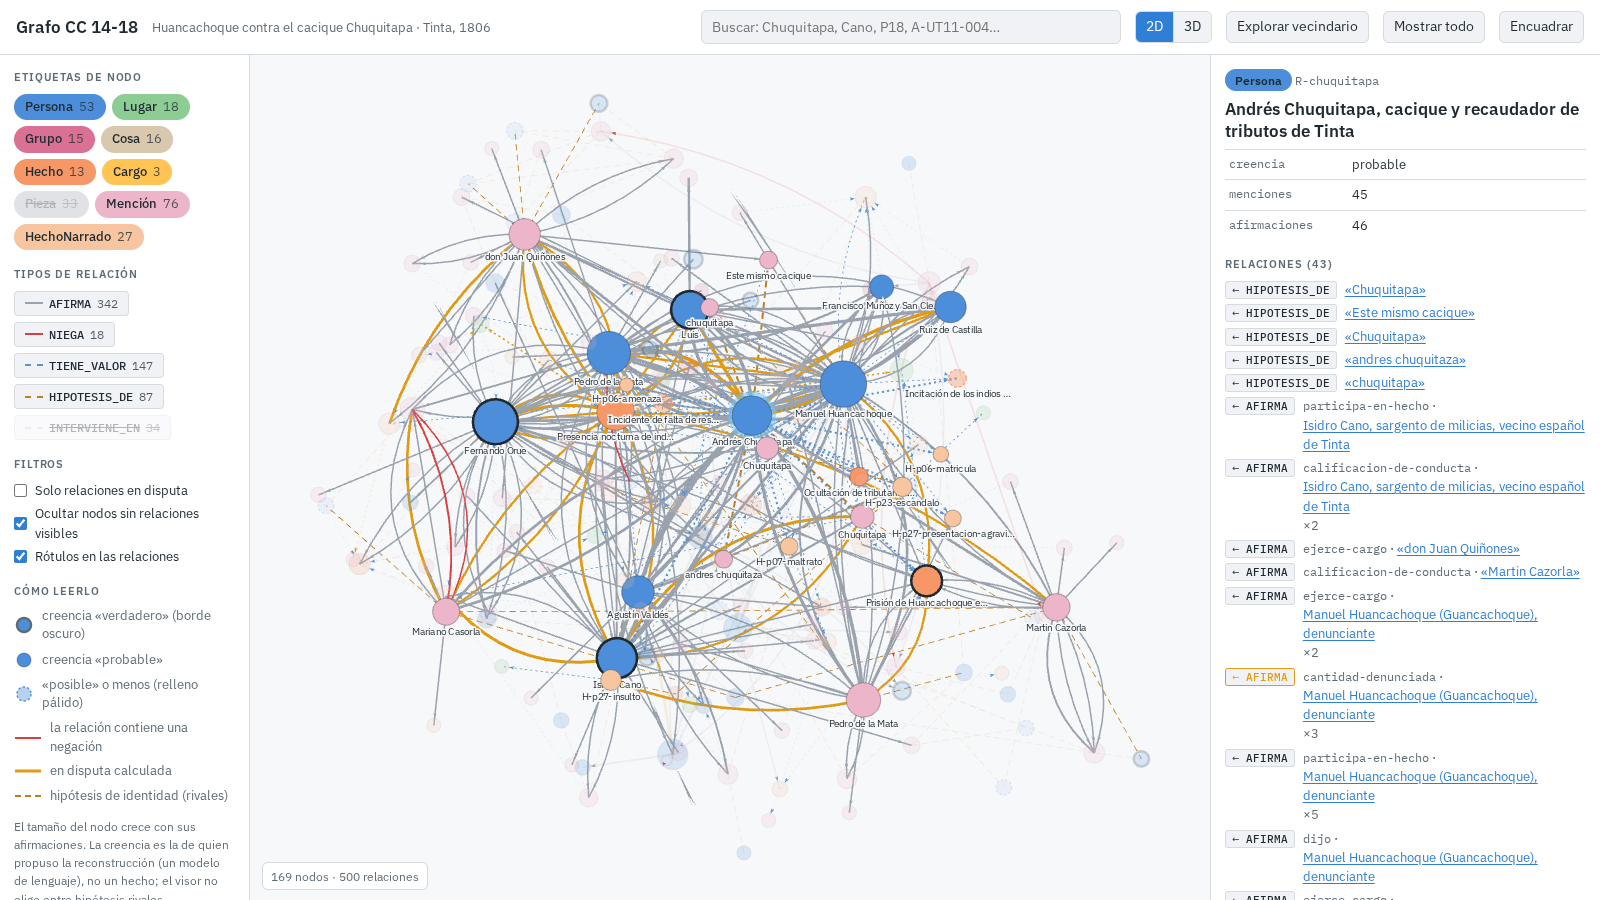
\includegraphics[width=\linewidth]{figuras/visor.png}

\scriptsize Visor (\ttt{visor/index.html}): Chuquitapa, sus 45 grafías y quién afirma qué de él.
\column{0.43\textwidth}
\small
\begin{itemize}\footnotesize
\item \textbf{Consultas}: 20 preguntas escritas \emph{antes} de modelar. Siete deben responder \alert{hay disputa} o
      \alert{no consta}, y lo hacen.
\item \textbf{Disputas calculadas}: se afirma y se niega lo mismo (coronel / no coronel), o se dan valores
      incompatibles (cuánto tiempo estuvo preso).
\item \textbf{Visor}: personas, lugares y cargos; aristas \emph{afirma} y \emph{niega}, en disputa resaltadas.
\item \textbf{Agente}: un modelo de lenguaje responde en castellano usando solo el grafo; un verificador rechaza
      citas que no estén en los datos. Sin citas inventadas en \cifra{\mediaVerificada} de 20 respuestas; completo
      en lo esencial en \cifra{\mediaEsencial}.
\end{itemize}
\end{columns}
\end{frame}

% ---------------------------------------------------------------------
\begin{frame}{Estado y en qué necesitamos su ayuda}
\begin{columns}[T]
\column{0.48\textwidth}
\small
\textbf{Hecho}
\begin{itemize}\footnotesize
\item Ontología OHAC, tesauro y reglas.
\item Expediente piloto completo y validado técnicamente.
\item Visor, consultas y un agente de consulta en pruebas.
\item Artículo sobre la ontología en borrador.
\end{itemize}
\textbf{Límites}
\begin{itemize}\footnotesize
\item Un solo expediente real.
\item Nada validado aún por un historiador.
\item Sin imágenes: el folio de cada pasaje no consta.
\end{itemize}
\column{0.5\textwidth}
\small
\textbf{Su ayuda}
\begin{enumerate}\footnotesize
\item Revisar una muestra de afirmaciones: ¿quién dijo qué, con qué fuerza?
\item Tesauro: las \cifraDefinicionesDeTrabajo{} definiciones de trabajo y los \cifraCandidatos{} candidatos.
\item Hipótesis de identidad, empezando por las rivales.
\item La transcripción del segundo expediente (CO Cusco L70 E15).
\item Preguntas que ustedes le harían al expediente.
\end{enumerate}
\end{columns}
\end{frame}

\begin{frame}[standout]
El grafo guarda \alert{quién afirmó qué};\\ no decide quién tiene razón.\\[8pt]
Gracias. ¿Preguntas?
\end{frame}

\end{document}
